\chapter{基于反事实多智能体学习的图像场景图生成方法}

图像场景图(scene graph)是将图像中每个物体当成一个节点,两两物体之间的视觉关系看成节点间的有向边,即视觉三元组“主语(物体)$\to$谓语(视觉关系)$\to$宾语(物体)”。图像场景图描绘了整个图像视觉场景中所有物体的类别、位置以及物体间的交互。为了生成准确的场景图,现有的场景图生成方法几乎都是通过“信息传递机制”(message passing),让每个物体和视觉关系都能充分地考虑和融合周围的视觉信息。例如,物体“人”和物体“自行车”之间一个最常见的视觉关系就是“骑”(即“人$\to$骑$\to$自行车”);同样,视觉关系“骑”也能够提升这两个物体(“人”和“自行车”)的类别预测概率。最后,这些方法都是直接利用物体和视觉关系分类的交叉熵之和作为模型最终的优化目标。然而,这个优化目标(交叉熵之和)将所有节点分类的重要性看成完全相同,即每个不同节点的分类损失对总的损失函数影响相同,这将大大限制模型融合周围信息的能力。

在本章,我们提出一种全新的反事实多智能体学习方法(Counterfactual critic Multi-Agent Training, CMAT)。模型CMT是一种基于多智能体策略梯度优化方法。它通过将每个物体看成一个智能体,从而将图像场景图生成任务转换成一个多智能体协同决策问题。基于这种转换,模型CMAT就可以直接利用整体场景图的生成质量作为优化目标(即全局奖励函数)。与此同时,为了给每个智能体分配适当的奖励,我们设计来一个反事实基准模型(counterfactual baseline)。这个反事实基准模型通过改变目标智能体的预测类别,同时固定其他所有智能体的预测,来推测当前智能体预测的局部贡献。通过在图像场景图生成数据集Visual Genome上进行大量的对比实验,模型CMAT在多个设定和评价指标下都达到当时最好的性能。


\section{问题描述}

视觉场景理解是计算机视觉研究领域一个重要的研究领域。它不仅仅需要对场景中所有物体的类别以及位置进行预测,同时需要对两两物体之间的视觉关系进行预测。随着目标检测~\cite{ren2015faster,liu2016ssd}与物体分割技术~\cite{long2015fully,he2017mask}的成熟,计算机已经可以准确地识别物体的类别、位置以及属性。然而,视觉场景理解不仅仅只是对单个物体的识别,还需要进一步对物体间视觉关系进行识别。所有的物体和视觉关系组合在一起,就构成了场景图~\cite{johnson2015image}。如图~\ref{ch4:fig:sgg}所示,场景图中每个节点和边分别表示图像中的物体和对应物体间的视觉关系。与此同时,图像场景图通常作为一种结构化的视觉知识,辅助许多视觉场景理解任务,如:图像描述生成~\cite{yao2018exploring,yang2019auto,kim2019dense}、视觉问答~\cite{norcliffe2018learning,hudson2019gqa}和视觉推理~\cite{shi2019explainable,haurilet2019s}等。

\begin{figure}[t]
    \centering
    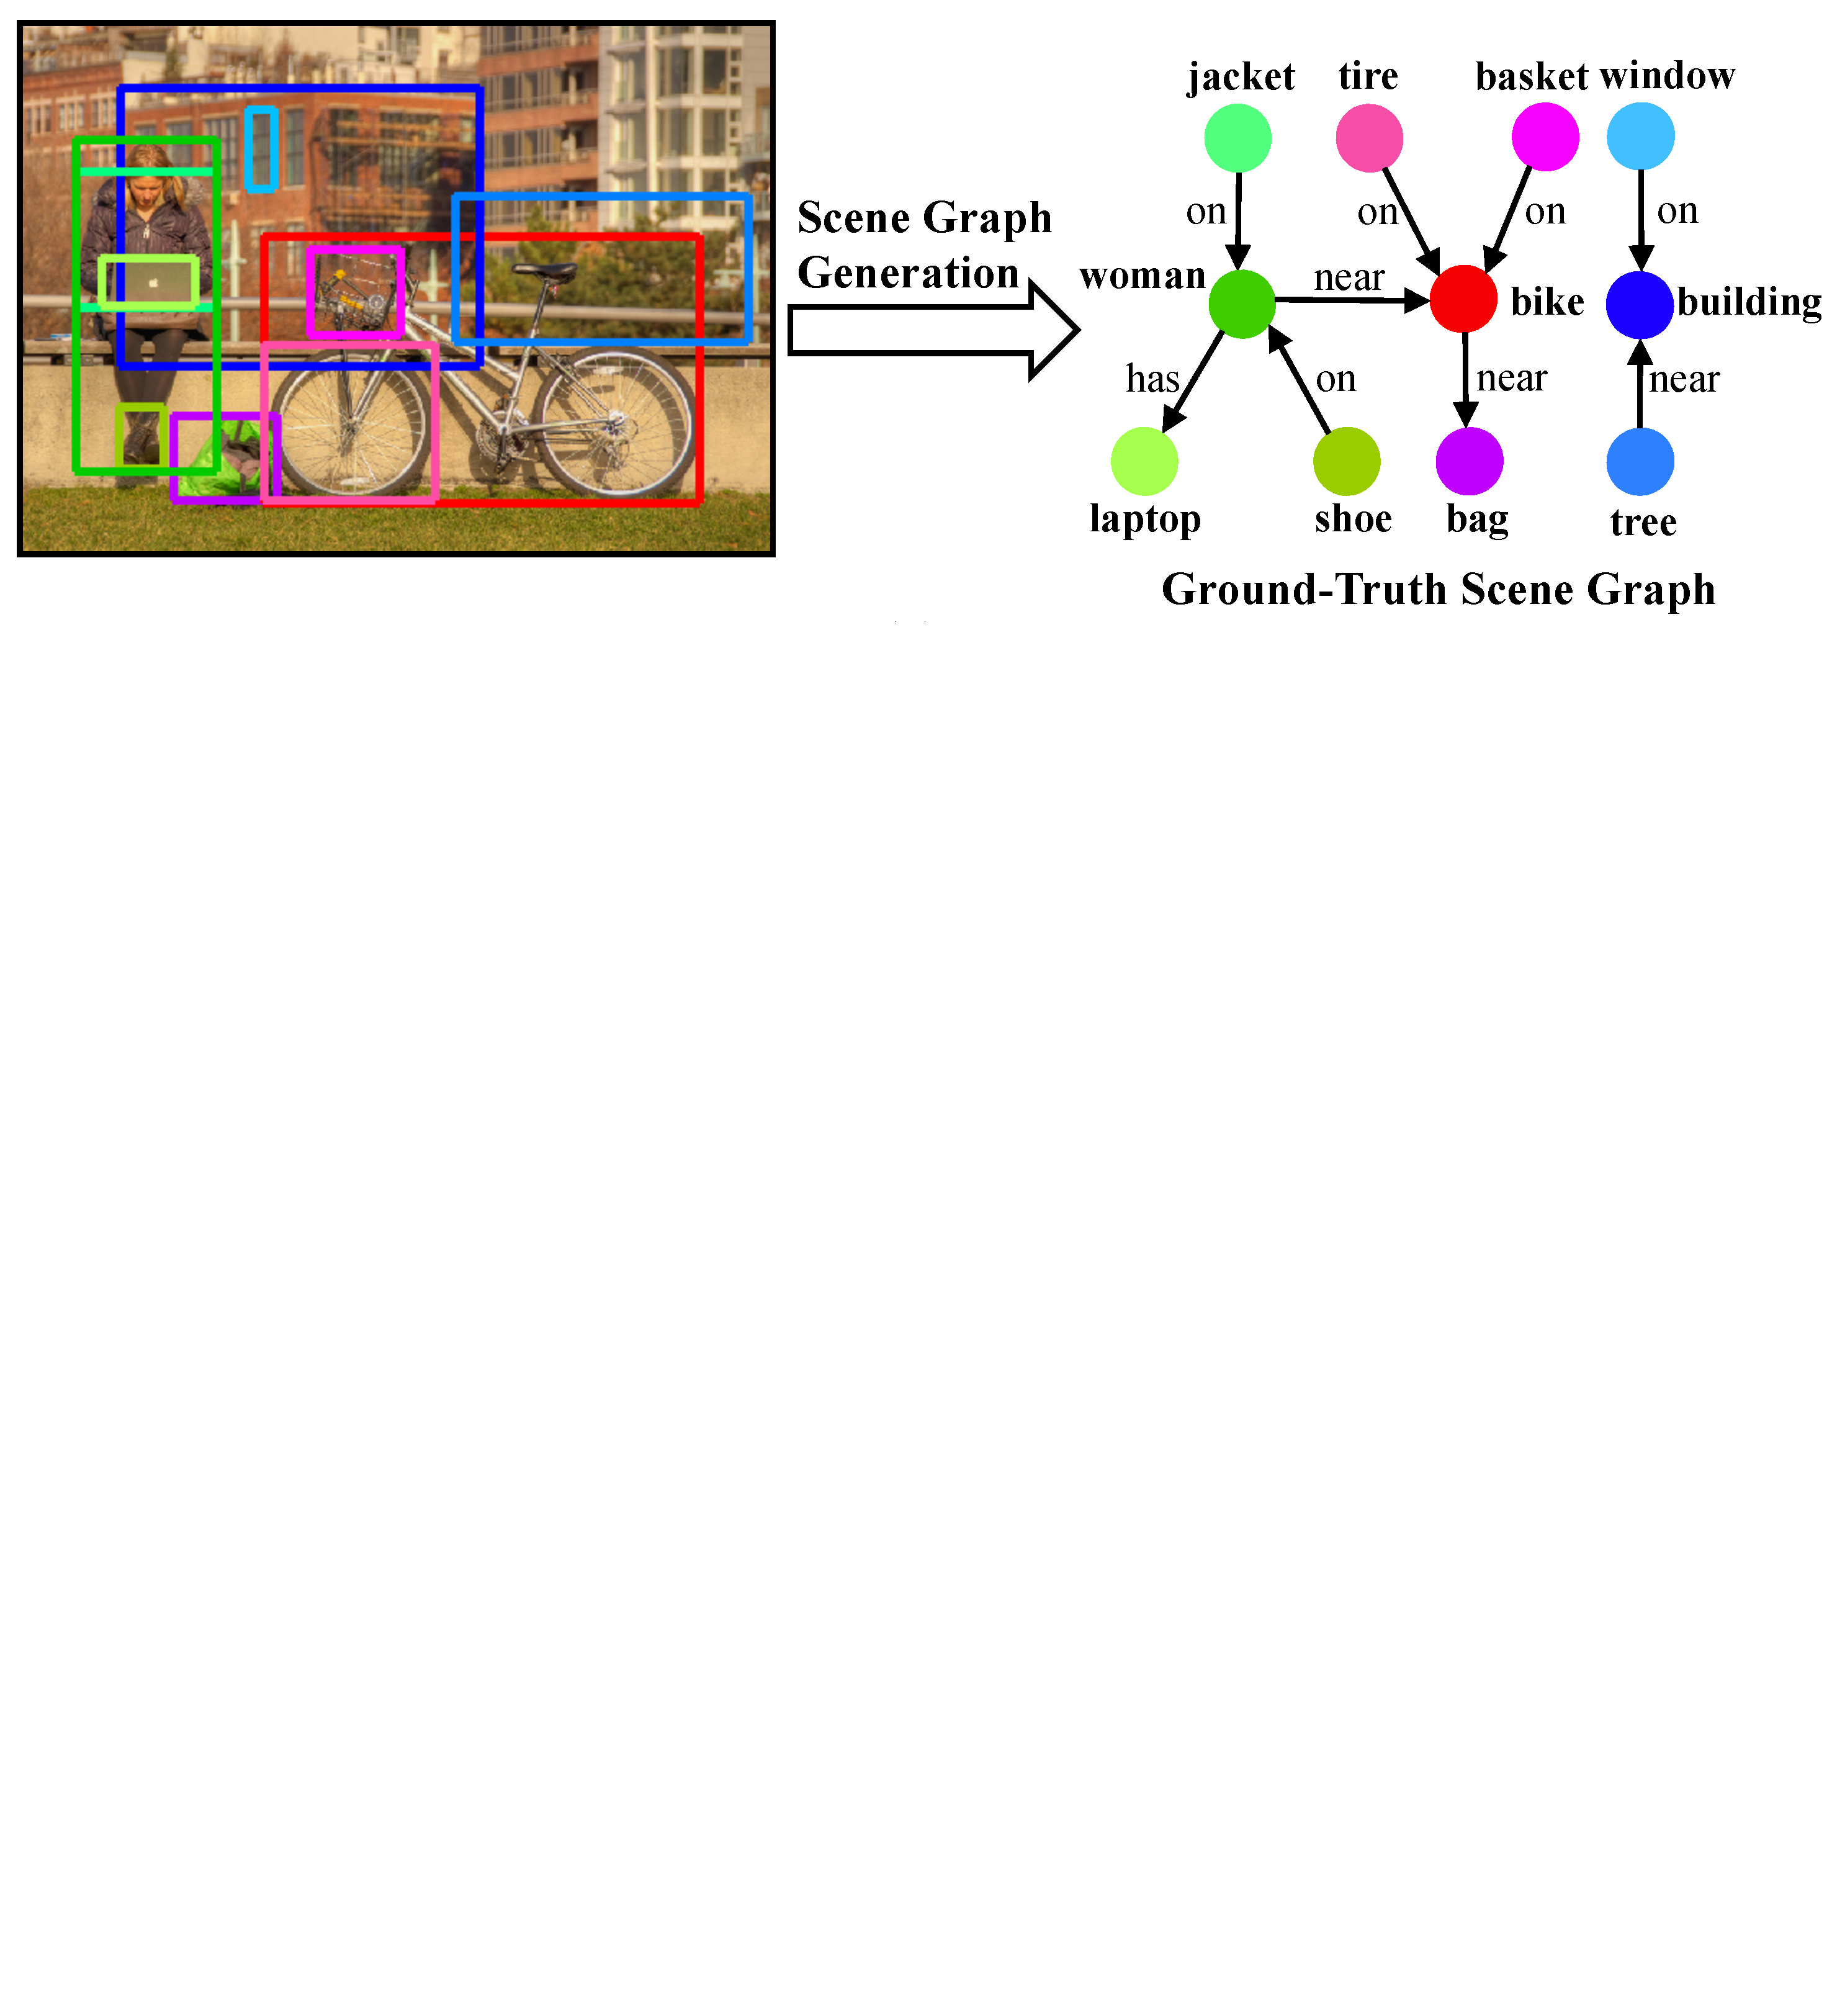
\includegraphics[width=0.95\linewidth]{chapter4/res/sgg.pdf}
    \caption{图像场景图生成任务示例}
    \label{ch4:fig:sgg}
\end{figure}

对于图像场景图生成任务(Scene Graph Generation, SGG),一个最直接的解决思路就是将场景图生成任务分解成物体分类和视觉关系分类两个独立的子任务,即先用一个物体检测器定位出物体框,然后分别预测每个物体框的类别以及两两物体框之间视觉关系的类别~\cite{lu2016visual,zhang2017visual,yang2018shuffle}。尽管这类方法的结构十分简单,但是它们都忽略了图像中所有视觉元素之间的内在联系,即每个物体(视觉关系)周围的视觉信息往往会提供一些归纳偏置~\cite{divvala2009empirical}(inductive bias)来辅助物体(视觉关系)的预测。如图~\ref{ch4:fig:sgg}所示,物体“窗户”(window)和物体“建筑物”(building)常常会出现在同一张图像中,“在附近”(near)也是物体“树”(tree)和物体“建筑物”(building)之间最常见的视觉关系类别。因此,从视觉关系三元组“窗户$\to$在上面$\to$?”或“树$\to$在附近$\to$?”中,很容易推测出物体“?”是“建筑物”。这些归纳偏置带来的辅助信息已经被广泛地用来提升场景图生成性能~\cite{xu2017scene, dai2017detecting, li2017vip, li2017scene, li2018factorizable, yin2018zoom, jae2018tensorize, zellers2018neural, tang2019learning, gu2019scene, qi2019attentive, wang2019exploring, qian2019video}。具体来说,这些方法都是通过借助条件随机场~\cite{zheng2015conditional}(Conditional Random Field, CRF)来建模所有节点和边的联合分布,然后通过信息传递机制来更新节点和边的特征~\cite{krahenbuhl2011efficient}。最后,整个模型利用所有节点(物体)和边(视觉关系)分类的交叉熵之和作为模型的优化目标进行参数优化。

\begin{figure}[t]
    \centering
    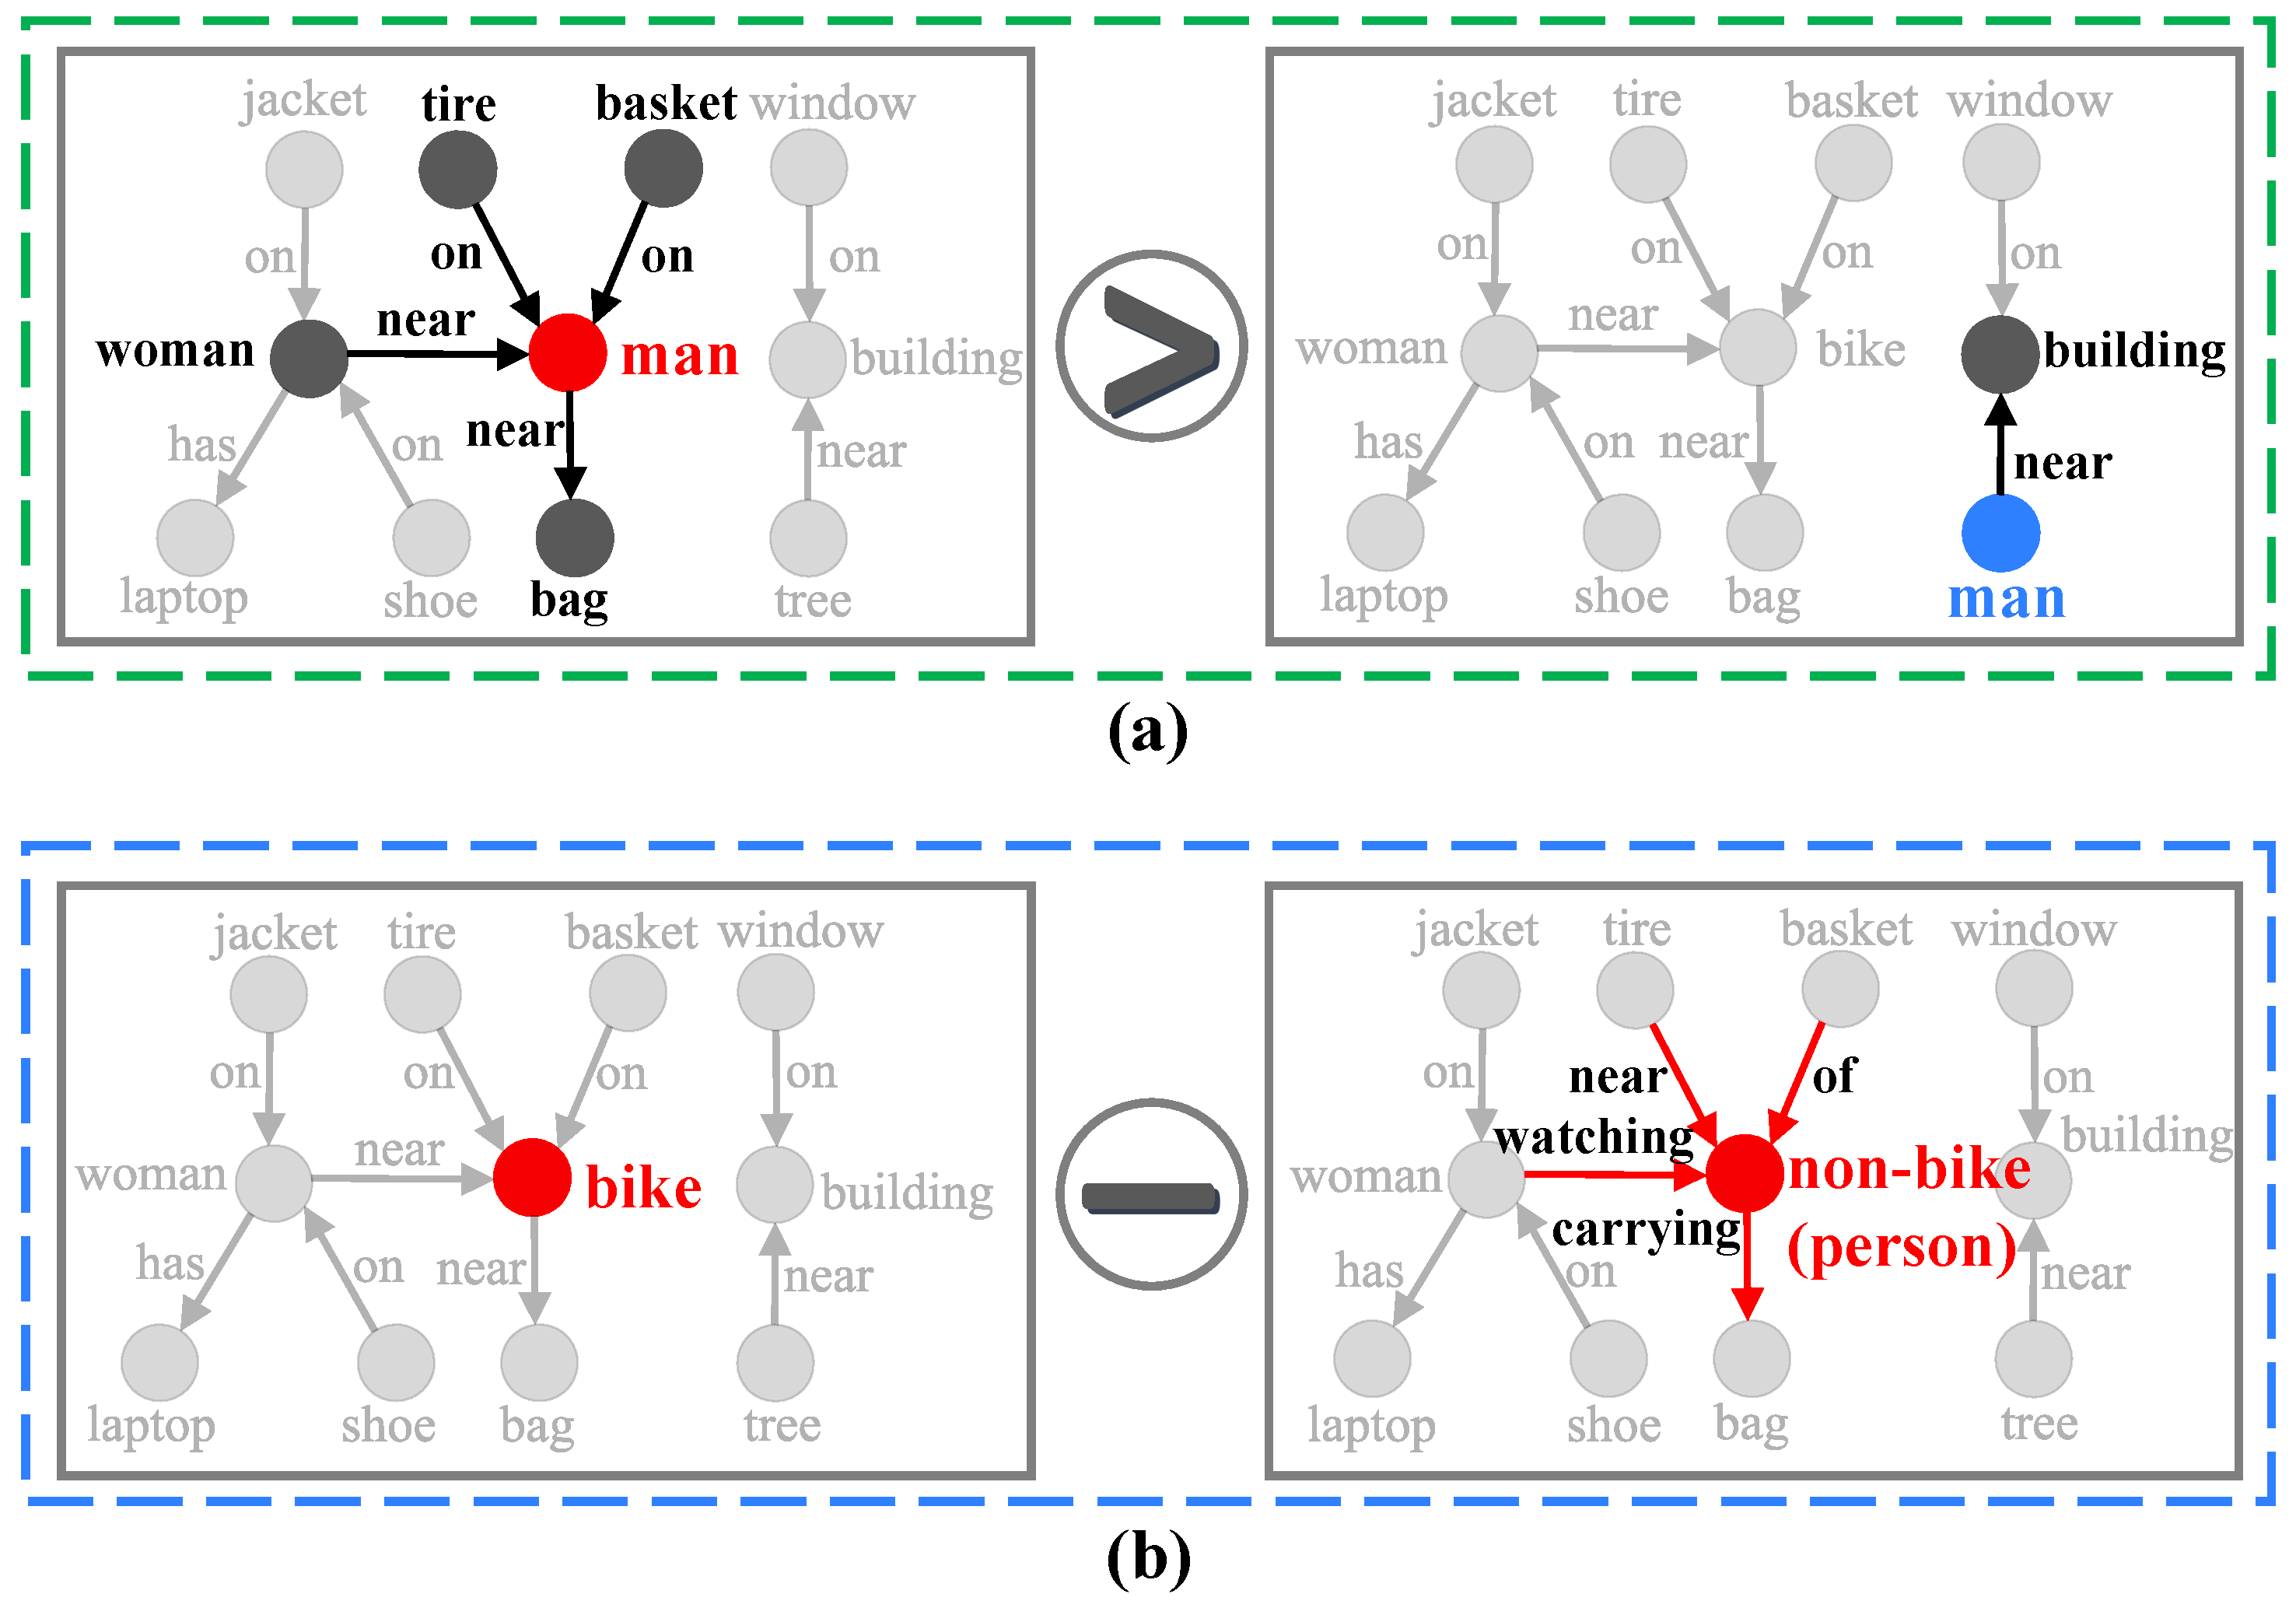
\includegraphics[width=0.95\linewidth]{chapter4/res/motivation.pdf}
    \caption{场景图生成中优化目标的整体一致性和局部敏感性}
    \label{ch4:fig:motivation}
\end{figure}

现有的图像场景图生成方法没有充分地利用场景中视觉元素之间的内在联系,一个重要的原因就是将物体和视觉关系分类的交叉熵之和作为场景图生成的优化目标。这个优化目标不具备\textbf{整体一致性}。所谓的“整体一致性”是指所有预测的物体类别和视觉关系类别之间应该保持整体一致。而交叉熵之和将所有的物体和视觉关系的预测看成是相互独立的。如图~\ref{ch4:fig:motivation}(a)所示,考虑两种极端情形,分别只有红色节点(“bike”)或蓝色节点(“tree”)被错误地分类成同一类别“man”,而其他所有的物体和视觉关系都正确。对于这两种情况,根据交叉熵之和的损失函数,它们最终的损失大小是完全相同的。然而,因为红色节点连接的边远多于蓝色节点,即对红色节点的错误分类将影响更多的视觉关系。因此,错误分类红色节点相比于错误分类蓝色节点应该导致更大的损失。因此,我们提出直接使用Recall@K~\cite{lu2016visual}或者SPICE~\cite{anderson2016spice}等图像场景图的全局评价指标作为优化目标。另一方面,场景图生成的优化目标还应该具备\textbf{局部敏感性}。所谓的“局部敏感性”是指优化目标应该能够感知每个节点类别的预测影响。由于场景图的全局评价指标是一个整体生成质量的评价数值,忽略了单个节点的预测贡献。因此我们需要设计一种机制,可以分解出每个节点各自预测的贡献,进而为每个局部预测计算更加有效的优化梯度。

在本章,我们提出了一种全新的场景图优化模型,可以同时满足优化目标的整体一致性和局部敏感性:反事实多智能体学习(CMAT)。具体来说,我们将图像场景图生成任务转换成一种多智能体协同决策任务。其中将每个物体看成是一个智能体,每个智能体的动作空间是所有可选择的物体类别。每个智能体之间可以进行通信,来编码周围的视觉元素,提升智能体内部的特征表达。经过多轮智能体通信之后,我们再利用一个视觉关系预测模型来预测智能体之间的视觉关系,得到最终的场景图预测结果。通过与人工标注的场景图对比,得到一个全局的奖励。

为了优化目标的整体一致性,我们直接将整体场景图生成的评价指标(如:Recall@K或SPICE~\cite{anderson2016spice})作为全局奖励函数,并且使用策略梯度(policy gradient)的方法对参数进行优化~\cite{sutton2000policy}。从多智能体强化学习~\cite{tampuu2017multiagent,lowe2017multi}(Multi-Agent Reinforcement Learning, MARL)的观点来看,尤其是“演员-评论家”方法~\cite{lowe2017multi}(actor-critic),模型CMAT模型中视觉关系预测模型可以看成是评论家(critic),而物体类别的分类模型可以看成是策略网络(policy network)。为了优化目标的局部敏感性,对于每个智能体,我们都从全局奖励中减去一个特定的反事实基准~\cite{foerster2018counterfactual}。这个反事实基准模型通过改变目标智能体的预测类别同时固定其他智能体的预测类别,来推测目标智能体预测的局部贡献。如图~\ref{ch4:fig:motivation}(b)所示,为了得到红色节点预测为“自行车”(bike)的贡献,我们可以固定其他节点的预测,而将红色节点的预测替换成其他的“非自行车”(non-bike)类,如“人”(person)等。进而通过计算出这种反事实式的替换对整体的场景图生成效果带来多大的影响,推测红色节点预测为“自行车”类别的贡献。

为了更好地编码物体周围的视觉元素信息和物体间的内在联系,我们还设计了一种更加有效的智能体通信(agent communication)模型。相比于现有的信息传递机制~\cite{xu2017scene, li2017scene, jae2018tensorize, li2017vip, yin2018zoom, li2018factorizable},我们不再将视觉关系也看成节点进行信息传递和更新。基于这个设计,我们可以将智能体通信与视觉关系分类两个任务分离出来,让前者关注如何编码物体周围视觉元素的内在联系,让后者作为评论家(critic)提供全局奖励来引导整个模型的优化。

我们在目前最大的图像场景图生成数据集Visual Genome上对模型CMAT的性能进行了验证。通过大量的对比实验,我们在通用的三种不同的实验设定下都可以达到当时最好的效果。

在本章,我们主要有三个技术贡献:

1)我们提出了一种全新的图像场景图生成模型的训练方法:反事实多智能体学习(CMAT)。据我们了解,我们是第一次将图像场景图生成任务转换成一个多智能体协同决策问题,使得优化目标满足整体一致性要求。

2)我们设计了一个全新的反事实基准模型,可以使得多智能体策略梯度算法的优化目标同时具备局部敏感性。

3)我们设计了一个有效的多智能体通信模型,有效地将智能体通信与视觉关系预测两个任务分离出来。


\section{反事实多智能体学习}
给定一个物体类别集$\mathcal{C}$(包括背景)和一个视觉关系类别集$\mathcal{R}$(包括没有视觉关系),图像场景图可以表示成:$\mathcal{G} = \left\{ \mathcal{V}=\{(v_i, \bm{l}_i)\},\mathcal{E}=\{r_{ij}\} | i,j = 1...n \right\}$,其中$\mathcal{V}$和$\mathcal{E}$分别表示所有节点(物体)和边(视觉关系)的集合。$v_i \in \mathcal{C}$表示第$i$个节点的物体类别,$\bm{l}_i \in \mathbb{R}^4$表示第$i$个节点的物体位置,$r_{ij} \in \mathcal{R}$表示第$i$个节点和第$j$个节点之间的视觉关系。图像场景图生成任务就是检测出图像中所有的物体以及物体间的视觉关系。

在本节,我们先介绍模型CMAT中的每个组成部分。然后,我们再介绍模型CMAT的优化目标。

\begin{figure}[t]
    \centering
    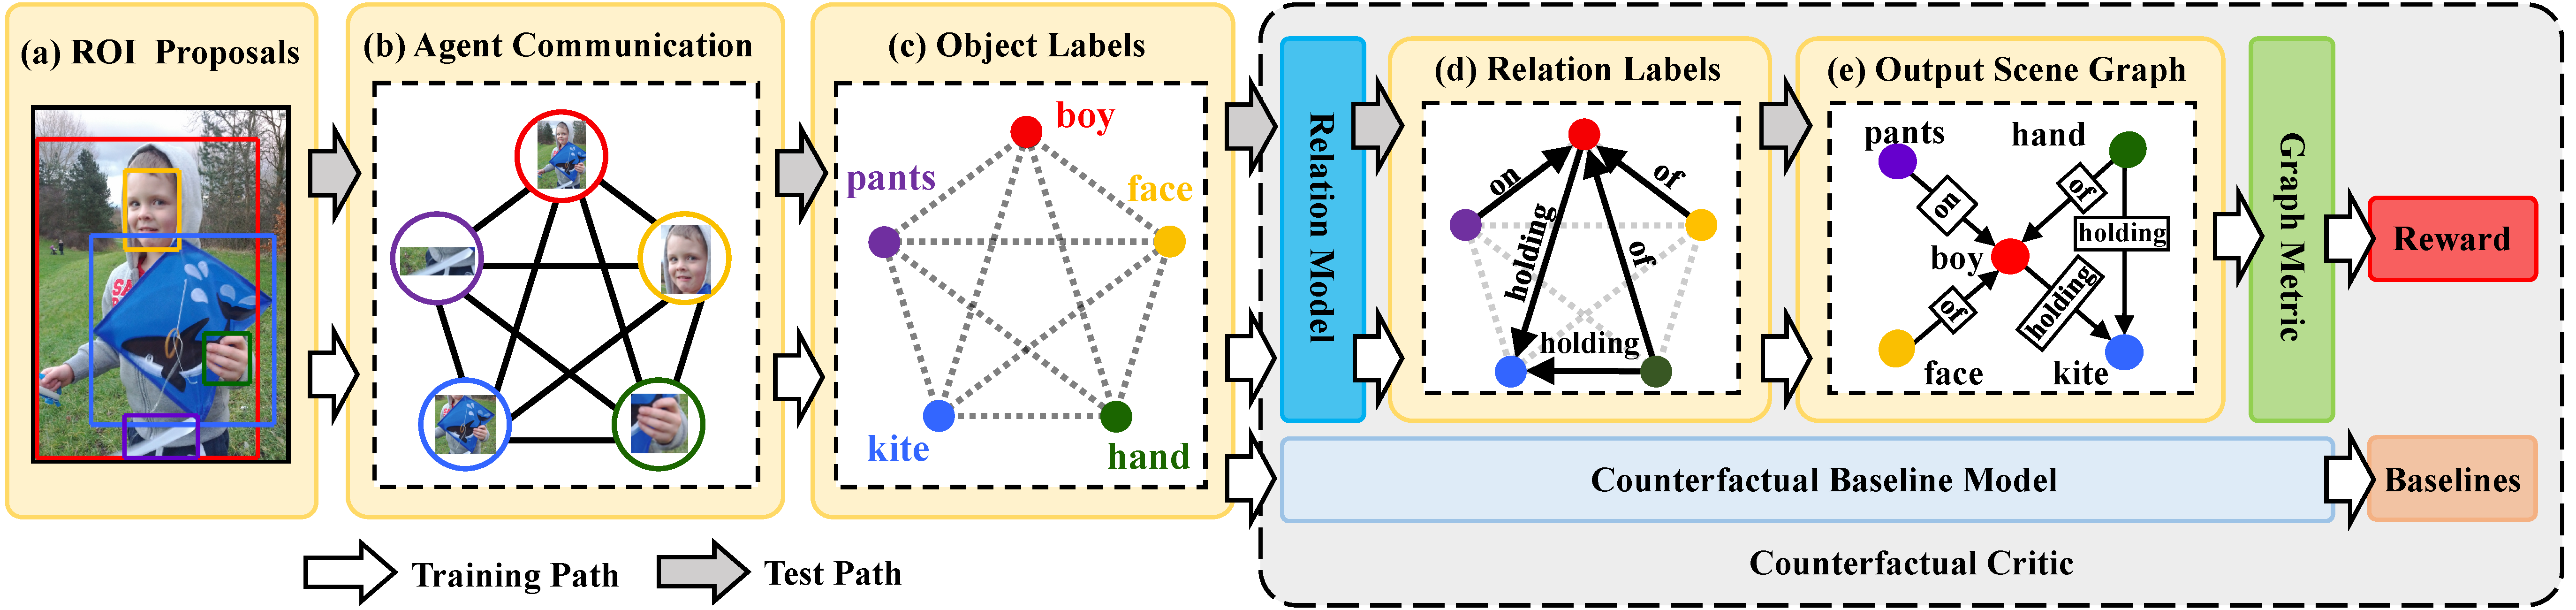
\includegraphics[width=\linewidth]{chapter4/res/architecture.pdf}
    \caption{模型CMAT的总体流程图}
    \label{ch4:fig:architecture}
\end{figure}

\subsection{多智能体协同决策模型}

\textbf{\kaishu{物体候选框检测}}:我们首先使用预训练好的目标检测器Faster R-CNN~\cite{ren2015faster}对输入图像进行物体检测,得到一系列候选框。对于每个候选框,我们可以同时得到其位置坐标$\bm{l}_i$、特征向量$\bm{x}^0_i$、以及初始的物体类别预测概率分布$\bm{s}^0_i$。上角标$0$表示$T$轮智能体通信的初始输入(第0轮)。我们参考现有的场景图生成工作~\cite{xu2017scene, zellers2018neural},固定所有候选框的位置$\{\bm{l}_i\}$作为物体位置的最终预测结果。为了后续表达的简洁性,我们在后续内容中省略位置坐标$\bm{l}_i$。


\textbf{\kaishu{智能体通信}}:给定$n$个物体候选框,我们将每个候选框看成是一个智能体。智能体之间将通过$T$轮的通信来编码每个物体与各自周围的视觉元素之间的内在联系。如图~\ref{ch4:fig:communication}所示,在单步智能体通信过程中,共有三个模块参与智能体通信:信息提取模块(extract module)、信息合成模块(message module)和状态更新模块(update module)。为了减小整个CMAT模型的参数量,这三个模块在所有的智能体之间都共享参数。关于这三个模块的具体细节如下:

\begin{figure}[t]
    \centering
    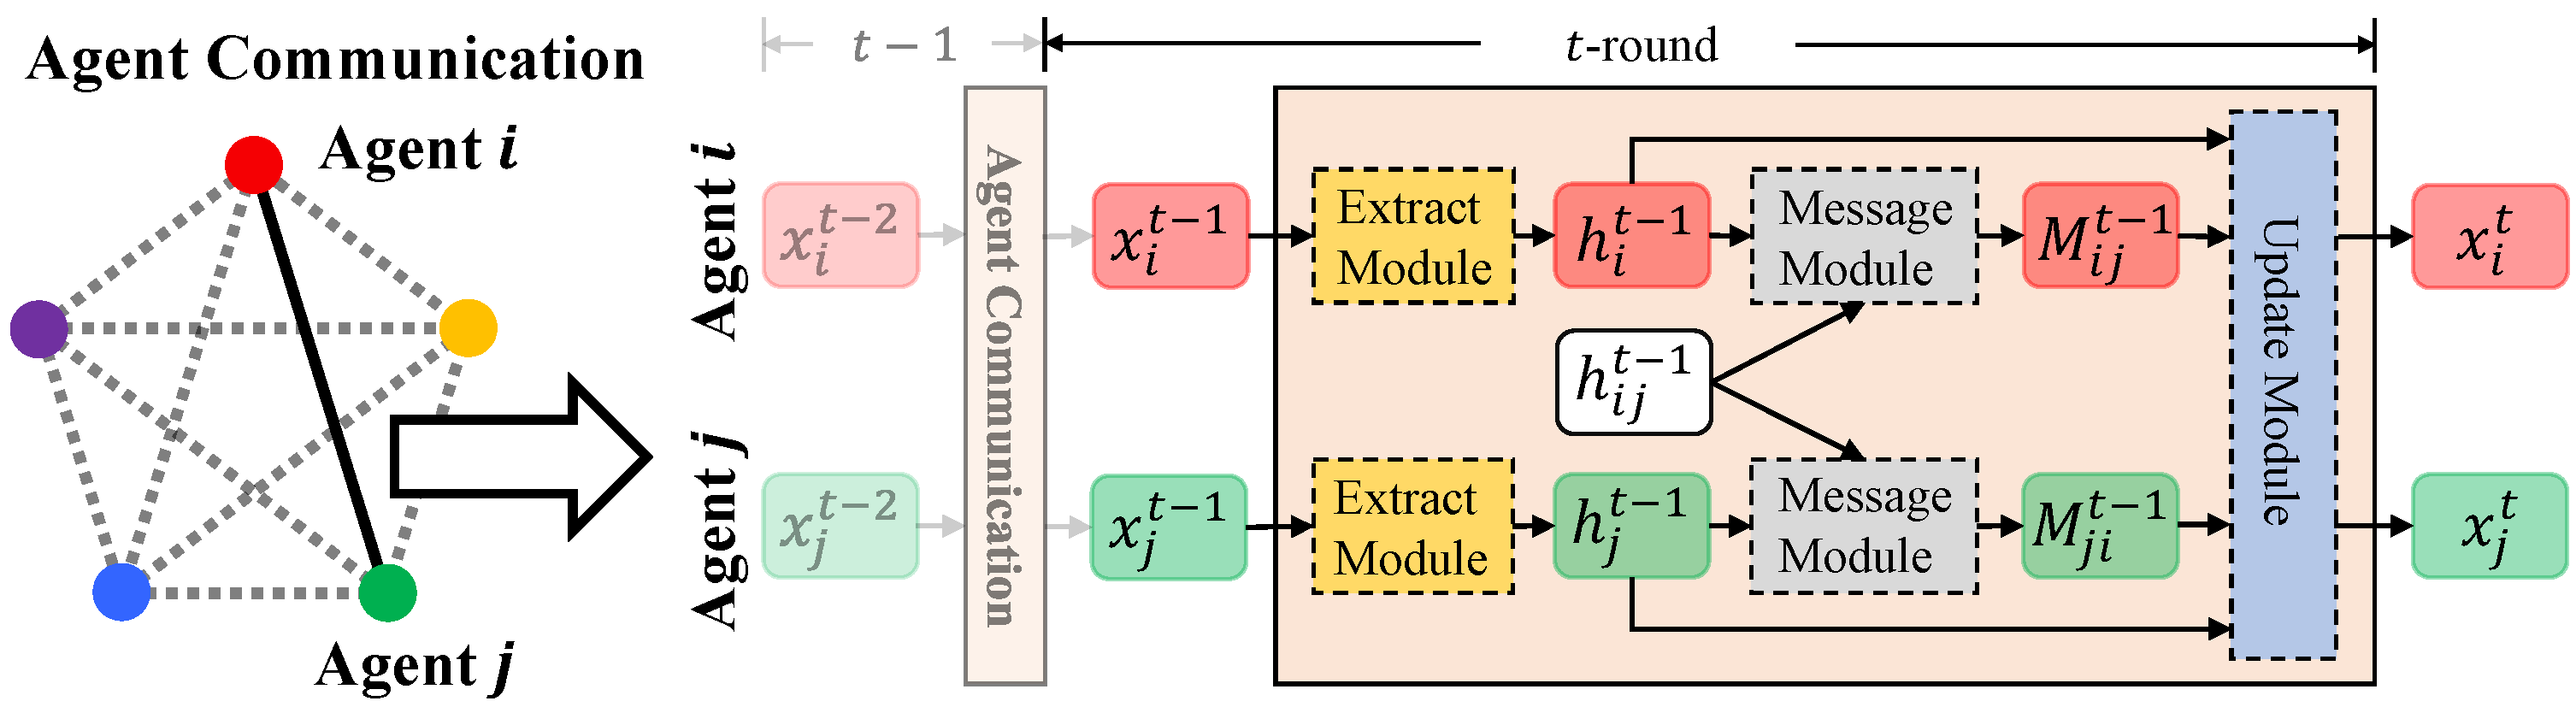
\includegraphics[width=\linewidth]{chapter4/res/communication.pdf}
    \caption{模型CMAT中的单步智能体通信示意图}
    \label{ch4:fig:communication}
\end{figure}

(a)信息提取模块:我们使用递归神经网络LSTM~\cite{hochreiter1997long}来实现信息提取模块。LSTM不仅可以编码智能体之间的交互历史,同时也可以提取智能体自身的内部状态。具体来说,对于第$i$个智能体,在第$t$轮($0 < t \leqslant T$)通信时:
\begin{equation}
\begin{aligned}
    \bm{h}^{t}_i & = \text{LSTM}(\bm{h}^{t-1}_i, [\bm{x}^{t}_i, \bm{e}^{t-1}_i]), \\
    \bm{s}^t_i & = \bm{s}^{t-1}_i + \bm{W}_h \bm{h}^{t}_i, \\
    v^t_i & \sim \bm{p}^{t}_i = \text{softmax}(\bm{s}^t_i), \\
    \bm{e}^{t}_i &= \textstyle{\sum_{\tilde{v}}} \bm{p}^{t}_i(\tilde{v}) \mathbf{E}[\tilde{v}],
\end{aligned}
\end{equation}
其中$\bm{h}^t_i \in \mathbb{R}^h$是LSTM的隐含状态向量,$\bm{x}^t_i \in \mathbb{R}^d$是每个LSTM时刻的输入特征,$\bm{s}^t_i \in \mathbb{R}^{|\mathcal{C}|}$是预测的物体类别概率分布。初始的(即第0步通信时)输入特征和类别预测概率都来自于物体候选框检测。$\mathbf{E}[\tilde{v}] \in \mathbb{R}^e$是类别标签$\tilde{v} \in \mathcal{C}$的特征编码向量,以及$\bm{e}^{t}_i \in \mathbb{R}^e$是一个基于类别概率$\bm{p}^t_i$加权的类别标签编码向量,$\bm{W}_h \in \mathbb{R}^{h \times |\mathcal{C}|}$是一个可学习的映射矩阵,以及$[,]$是向量间的连接操作。所有的隐藏状态$\{\bm{h}^t_i\}$都输入到之后的信息合成模块用于合成通信信息。


(b)信息合成模块:对于第$i$个智能体和第$j$个智能体之间的通信,信息合成模块将分别合成信息$M^t_{ij}$和$M^t_{ji}$。具体来说,对于第$i$个智能体收到的信息$M^t_{ij} = (\bm{m}^t_j, \bm{m}^t_{ij})$,主要包含两部分:
\begin{equation}
\begin{aligned}
\bm{m}^t_j = \bm{W}_u \bm{h}^t_j, \; \bm{m}^t_{ij} = \bm{W}_p\bm{h}^t_{ij},
\end{aligned}
\end{equation}
其中$\bm{m}^t_j \in \mathbb{R}^h$表示一元信息,用来表征第$j$个智能体本身的属性(如:单个物体的局部视觉特征),$\bm{m}^t_{ij} \in \mathbb{R}^h$表示二元信息,用来表征两个智能体之间的交互信息(如:两个智能体的相对位置信息)。$\bm{h}^t_{ij} \in \mathbb{R}^d$表示第$i$个智能体与第$j$个智能体之间的共同特征,它的初始化是两个智能体物体框合并之后的视觉特征。对于第$i$个智能体,所有来自其他智能体的通信信息$\{M^t_{i*}\}$和其内部状态$\bm{h}^t_i$都输入到状态更新模块,更新其内部状态。

(c)状态更新模块:在每轮智能体通信过程中,对于每个智能体,我们使用注意力机制~\cite{chen2017sca}来融合不同智能体的通信信息:
\begin{equation}
\begin{aligned}
    u^t_j &= \bm{w}_u [\bm{h}^t_i, \bm{h}^t_j], \\ 
    u^t_{ij} &= \bm{w}_p [\bm{h}^t_i, \bm{h}^t_{ij}], \\
    \alpha^t_j & = \exp(u^t_j) / \textstyle{\sum_k} \exp(u^t_k), \\
    \alpha^t_{ij} & = \exp(u^t_{ij}) / \textstyle{\sum_k} \exp(u^t_{ik}), \\
    \bm{x}^{t+1}_i &= \bm{W}_x (\text{ReLU} (\bm{h}^t_i + \textstyle{\sum_j} \alpha^t_j \bm{m}^t_j +  \textstyle{\sum_j} \alpha^t_{ij} \bm{m}^t_{ij})), \\
    \bm{h}^{t+1}_{ij} &= \text{ReLU} (\bm{h}^t_{ij} + \bm{W}_s \bm{h}^{t+1}_i + \bm{W}_e \bm{h}^{t+1}_j),
\end{aligned}
\end{equation}
其中$\alpha^t_j$和$\alpha^t_{ij}$是不同信息融合的权重,$\bm{w}_u \in \mathbb{R}^{2h}$、$\bm{w}_p \in \mathbb{R}^{h+d}$、$\bm{W}_x \in \mathbb{R}^{h\times d}$、$\bm{W}_s \in \mathbb{R}^{h\times d}$和$\bm{W}_e \in \mathbb{R}^{h\times d}$这些都是需要学习的映射矩阵。


\textbf{\kaishu{视觉关系预测}}:在$T$轮智能体通信之后,所有的智能体都完成了状态更新。在测试阶段,对于所有的智能体,我们直接根据预测的分数$\bm{s}^T_i$来选取所有智能体的物体类别$v^T_i$。最后,我们再利用视觉关系预测模型对任意两个智能体之间进行视觉关系分类:
\begin{equation}
\begin{aligned}
    \bm{z}_i & = \bm{W}_o [\bm{h}^T_i, \mathbf{E}[v^T_i]], \\
    \bm{z}_j & = \bm{W}_o [\bm{h}^T_j, \mathbf{E}[v^T_j]], \\
    \bm{p}_{ij} & = \text{softmax} ([\bm{z}_i,  \bm{z}_j] \odot \bm{W}_r \bm{z}_{ij} + \bm{w}_{v^T_i, v^T_j}), \\
    r_{ij} & = \arg \textstyle{\max_{r \in \mathcal{R}}} \bm{p}_{ij}(r),
\end{aligned}
\end{equation}
其中$\bm{W}_o \in \mathbb{R}^{(h+e) \times z}$、$\bm{W}_r \in \mathbb{R}^{z\times 2z}$都是需要学习的映射矩阵,$\bm{z}_{ij} \in \mathbb{R}^z$是第$i$个智能体与第$j$个智能体之间预测的视觉关系特征,$\odot$是特征融合函数~\cite{zhang2018learning}: $\bm{x} \odot \bm{y} = \text{ReLU}(\bm{W}_x \bm{x} + \bm{W}_y \bm{y}) - (\bm{W}_x \bm{x} - \bm{W}_y \bm{y})^2$,$\bm{w}_{v^T_i, v^T_j} \in \mathbb{R}^{|\mathcal{C}|}$是基于VG数据集统计的视觉关系类别偏置~\cite{zellers2018neural}。 


\subsection{反事实多智能体学习}

在本节,我们将详细介绍模型CMAT中优化目标的细节,具体包括:(1)符合整体一致性的多智能体策略梯度算法;(2)符合局部敏感性的反事实评论家模型。


\textbf{\kaishu{优化目标的整体一致性}}:目前,几乎所有的场景图生成算法都是将所有物体和视觉关系分类的交叉熵之和作为模型的优化目标。对于一个预测的场景图($\hat{\mathcal{V}}, \hat{\mathcal{E}}$),如果人工标注的场景图为($\mathcal{V}^{gt}, \mathcal{E}^{gt}$),根据交叉熵之和(cross-entropy, XE)的优化目标,整个模型的损失函数则为:
\begin{equation} \label{ch4:eq:eq_5}
\begin{aligned}
   L(\theta) =  \textstyle{\sum_{ij}} \left(\text{XE}(\hat{v}_i, v^{gt}_i) + \text{XE}(\hat{r}_{ij}, r^{gt}_{ij}) \right). 
\end{aligned}
\end{equation}
由公式~\eqref{ch4:eq:eq_5}可以看出,交叉熵之和的优化目标本质上将所有的节点预测都看成相互独立的。

为了解决上述问题,我们提出将交叉熵之和的优化目标替换成以下两种具备整体一致性的优化目标:(1)\textbf{Recall@K}~\cite{lu2016visual}在预测分数最高的前K个视觉三元组(“主语$\to$谓语$\to$宾语”)中,预测正确的视觉三元组占所有标注视觉三元组的百分比。(2)\textbf{SPICE}~\cite{anderson2016spice}:所有视觉三元组预测的准确率和召回率之间的F值。与交叉熵之和不同的是,Recall@K和SPICE都是不可导的。因此,模型CMAT需要借助多智能体策略梯度算法对模型参数进行优化。


\textbf{\kaishu{多智能体策略梯度}}:
我们首先定义模型CMAT中智能体的动作(action)、策略函数(policy)和状态(state)。然后,我们推导出模型参数的梯度计算公式。

(a)动作:每个智能体的动作空间是所有可选择的物体类别的集合,即第$i$的智能体的动作是$v^t_i$。我们用集合$V^t = \{v^t_i\}$来表示所有智能体的动作集合。

(b)状态:我们参考Hausknecht等人~\cite{hausknecht2015deep}使用递归神经网络LSTM(信息提取模块)来编码智能体与环境之间的交互历史(history)。LSTM的隐含状态$\bm{h}^t_i$可以看成是第$i$个智能体对局部可见环境状态的近似。我们用集合$H^t = \{\bm{h}^t_i\}$来表示所有智能体的状态集合。

(c)策略函数:每个智能体的策略函数就是物体类别分类模型。在训练阶段,每个智能体通过对分类概率进行采样得到智能体类别,即:$\bm{p}^T_i = \text{softmax}(\bm{s}^T_i)$。因为模型CMAT只在$T$轮智能体通信之后进行动作采样,根据策略梯度的理论~\cite{sutton2000policy},模型CMAT中梯度计算公式为:
\begin{align}
\nabla_{\theta} J \approx \sum^n_{i=1} \nabla_{\theta} \log \bm{p}^T_i (v^T_i|h^T_i; \theta)Q(H^T, V^T),
\end{align}
其中,$Q(H^T, V^T)$为状态-动作函数(state-action value function)。不同于现有的演员-评论家~\cite{bahdanau2017actor,lowe2017multi,konda2000actor}(actor-critic)算法通常用一个独立的网络来近似函数$Q$,在模型CMAT中,我们参考Rao等人~\cite{rao2018learning}直接使用实际的奖励来代替函数$Q$。这样做的原因主要有两个:(1)在图像场景图生成任务中,智能体的数量(如:SGDet中通常检测64个物体框)和动作空间的采样大小(如:数据集VG中有150个物体类别)都明显大于现有的多智能体策略梯度的工作。这容易导致训练样本不充足,难以训练一个准确的状态-动作函数。(2)直接使用实际的奖励可以大大减小模型的复杂度,提升模型训练速度。因此,模型CMAT中梯度计算公式变为:
\begin{align} \label{ch4:eq:eq_7}
\nabla_{\theta} J \approx \sum^n_{i=1} \nabla_{\theta} \log \bm{p}^t_i (v^T_i|h^T_i; \theta) R(H^T, V^T),
\end{align}
其中,$R(H^T, V^T)$是实际的全局奖励(即:Recall@K或SPICE)。另外,值得注意的是,$R(H^T, V^T)$里包含一个可以学习的视觉关系分类模型。

\begin{figure}[t]
    \centering
        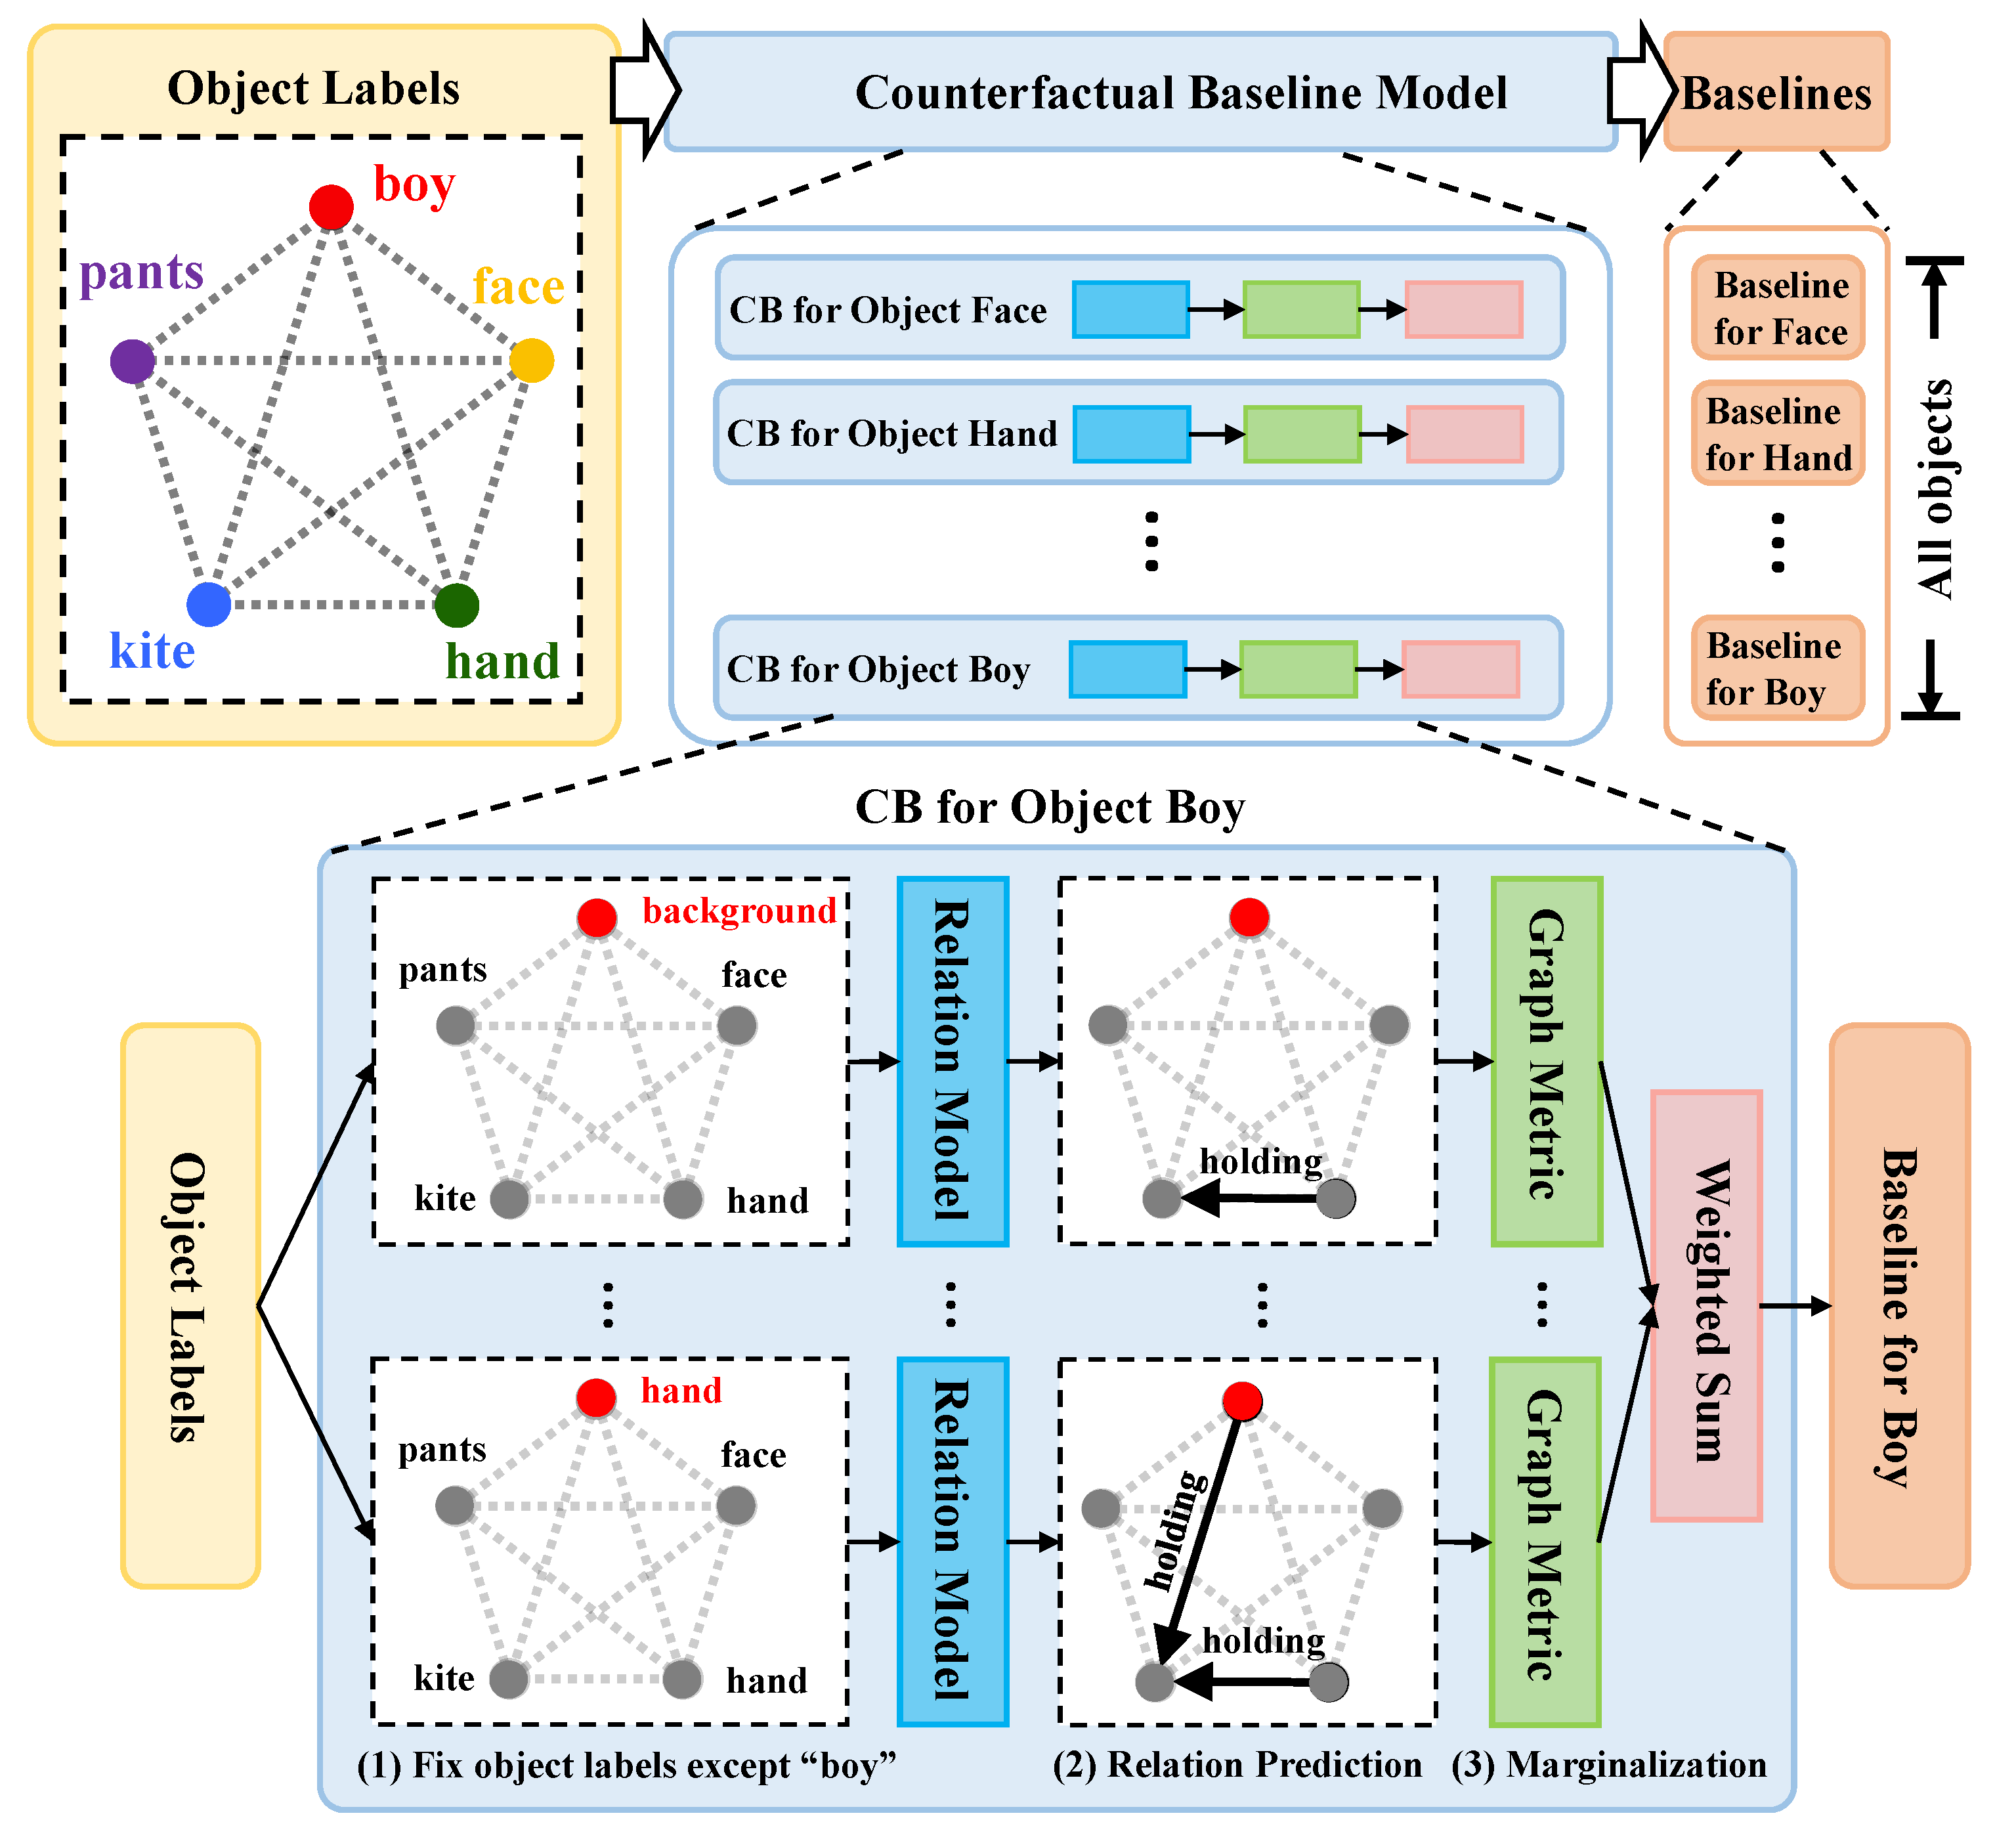
\includegraphics[width=0.95\linewidth]{chapter4/res/baseline.pdf}
    \caption{模型CMAT中反事实基准模型}
    \label{ch4:fig:baseline}
\end{figure}


\textbf{\kaishu{优化目标的局部敏感性}}:从上述公式~\eqref{ch4:eq:eq_7}可以看出,全局的奖励是综合考虑了所有智能体预测类别的总贡献,即对每个单独的智能体而言,总贡献是完全相同的。在图~\ref{ch4:fig:local_sensitive}中,我们用一个简单的示例来说明这种“总贡献”对场景图生成任务的副作用。如图~\ref{ch4:fig:local_sensitive}所示,绿色和红色分别表示正确的预测和错误的预测(包括节点和边),假定全局奖励函数定义为预测正确的视觉三元组数减去预测错误的视觉三元组数,且在图~\ref{ch4:fig:local_sensitive}(1)(2)两个场景图中只有节点“a”预测不同,其他预测都完全相同。

\begin{wrapfigure}{r}{0.55\linewidth}
    \centering
        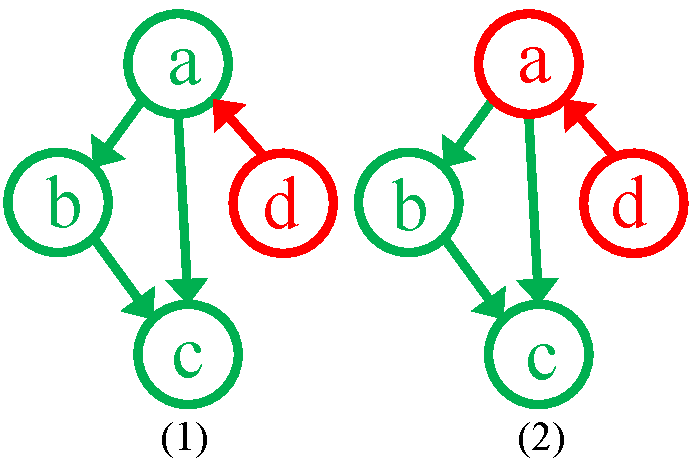
\includegraphics[width=0.9\linewidth]{chapter4/res/local_sensitive.pdf}
    \captionof{figure}{优化目标局部敏感性的重要性示例图}
    \label{ch4:fig:local_sensitive}
\end{wrapfigure}

根据公式~\eqref{ch4:eq:eq_7},场景图(1)中所有的节点都得到一个正的全局奖励(3-1=+2),而场景图(2)中所有的节点都得到一个负的全局奖励(1-3=-2)。在这两种情况下,虽然节点“b”、“c”、“d”的预测完全相同,但是对于它们计算得到的梯度方向却完全相反,容易造成模型多次无效的优化迭代。因此,通过让优化目标满足局部敏感性,即通过计算每个智能体各自的局部奖励,有利于提供更有效的优化梯度,提升模型训练效率。

\textbf{\kaishu{反事实评论家}}:一个直观地计算某个智能体动作的局部奖励的方法就是将目标智能体的动作替换成其他的动作,然后利用总贡献的变化来近似。因此,$R(H^T, V^T) - R(H^T, (V^T_{-i}, \tilde{v}^T_i))$可以表示第$i$个智能体的动作$v^T_i$的局部贡献,其中$V^T_{-i}$表示除第$i$个智能体以外其他所有智能体都保持初始的预测动作,而第$i$个智能体采取新的动作$\tilde{v}^T_i$。由于新的动作$\tilde{v}^T_i$有$|\mathcal{C}|$种可能性,为了准确地计算其他所有智能体动作(即:$V^T_{-i}$)的贡献,我们对所有可能的动作进行平均:$ \text{CB}^i(H^T, V^T) = \sum \bm{p}^T_i(\tilde{v}^T_i) R(H^T, (V^T_{-i}, \tilde{v}^T_i))$,其中$\text{CB}^i(H^T, V^T)$称为第$i$个智能体的\textbf{反事实基准}(counterfactual baseline)。这个反事实基准表示的意义是无论第$i$个智能体采用的动作,其他所有智能体采用默认动作时模型能够得到的平均全局奖励。模型CMAT的反事实基准模型展示在图~\ref{ch4:fig:baseline}中。

给定一个全局的奖励$R(H^T, V^T)$和第$i$个智能体动作的反事实基准$\text{CB}^i(H^T, V^T)$,我们可以得到第$i$个智能体动作的局部贡献为:
\begin{align}
    A^i(H^T, V^T) = R(H^T, V^T) - \text{CB}^i(H^T, V^T),
\end{align}
其中,$A^i(H^T, V^T)$在演员-评论家算法~\cite{sutton2018reinforcement,mnih2016asynchronous}中常被称为“优势”(advantage),$\text{CB}^i(H^T, V^T)$在策略梯度算法中常被称为“基准”(baseline),用来减少梯度计算时的方差。整个计算$A^i(H^T, V^T)$的网络结构可以合称为“反事实评论家”(counterfactual critic)。因此,根据公式~\eqref{ch4:eq:eq_7},模型CMAT的梯度计算公式变为:
\begin{align}
\nabla_{\theta} J \approx \sum^n_{i=1} \nabla_{\theta} \log \bm{p}^T_i (v^T_i|h^T_i; \theta) A^i(H^T, V^T).
\end{align}

最后,我们在加上交叉熵之和损失一起训练,最终参数训练的梯度为:
\begin{equation}
\begin{split}
\nabla_{\theta} J \approx  \overbrace{\sum^n_{i=1} \nabla_{\theta} \log \bm{p}^T_i (v^T_i|h^T_i; \theta) A^i(H^T, V^T)}^{\text{CMAT}} + \\
\underbrace{\alpha\sum^n_{i=1}\sum^n_{j=1} \nabla_{\theta} \log \bm{p}_{ij}(r_{ij})}_{\text{视觉关系交叉熵之和}} + 
\underbrace{\beta \sum^n_{i=1} \nabla_{\theta} \log \bm{p}^T_i(v^T_i)}_{\text{物体类别交叉熵之和}},
\end{split}
\end{equation}
其中,$\alpha$和$\beta$是不同损失函数之间权衡的权重,额外的交叉熵之和是为了增加模型训练的稳定性~\cite{rao2018learning}。同样,我们还增加了一个熵正则项~\cite{xu2015show, hu2017learning}来约束$\{\bm{p}^T_i\}_i$。


\section{实验设置与性能对比}
\subsection{图像场景图生成数据集与实验设定}

\textbf{\kaishu{图像场景图生成数据集}}:我们使用目前最大的图像场景图数据集Visual Genome~\cite{krishna2017visual}对模型性能进行评估。为了能够与现有的工作公平地进行比较,我们采用与它们完全相同的数据集划分和预处理步骤~\cite{xu2017scene, zellers2018neural, newell2017pixels, yang2018graph, herzig2018mapping}。处理后的数据集共包含150个物体类别和50个视觉关系类别。每张图像平均包含11.5个物体和6.2个视觉关系。在整个数据集中,70\%的图像作为训练集,剩余30\%的图像作为测试集。


\textbf{\kaishu{实验设定}}:我们参考现有的图像场景图生成的工作~\cite{xu2017scene, zellers2018neural, jae2018tensorize},在三种实验设定下评估场景图生成质量:
\begin{asparaenum}
\item \textbf{视觉关系分类(PredCls)}:给定图像中所有的物体框位置和物体类别,模型只需要预测两两物体间的视觉关系类别;

\item \textbf{场景图分类(SGCls)}:给定图像中所有的物体框位置,模型需要预测所有物体的类别以及两两物体间的视觉关系类别;

\item \textbf{场景图检测(SGDet)}:给定图像,模型需要检测物体框位置、预测物体类别以及两两物体间的视觉关系类别。
\end{asparaenum}

一个视觉三元组预测正确,不仅需要主语(subject)、谓语(predicate)和宾语(object)的类别都预测正确,同时需要主语和宾语的物体框与真实准确物体框的交并比(IoU)均大于0.5。按照图像场景图生成任务惯例,我们使用Recall@20(R@20)、Recall(R@50)和Recall(R@100)作为场景图生成质量的评价指标。

\subsection{实验细节}

\textbf{\kaishu{物体检测器}}:为了公平地与现有的工作进行对比,我们采用了与Zellers等人~\cite{zellers2018neural}完全相同的物体检测器。具体来说,它是以VGG网络~\cite{simonyan2015very}为主干网络,然后锚框的大小和长宽比与YOLO-9000~\cite{redmon2017yolo9000}设置一样, 然后用RoIAlign~\cite{he2017mask}代替RoIPooling~\cite{girshick2014rich,girshick2015fast}。

\textbf{\kaishu{训练细节}}:我们参照之前的策略梯度的工作,将整个训练过程分成两个阶段:先使用监督训练对模型参数进行初始化,再使用策略梯度对模型参数进行微调。在监督训练过程中,我们将RoIAlign层之前的参数都固定住,然后使用所有物体和视觉关系分类的交叉熵之和作为优化目标。批处理的大小和初始的学习率分别设为6和$10^{-3}$。在策略梯度优化过程中,初始的学习率设为$3\times5^{-5}$。对于场景图检测任务,因为所有可能的物体组合非常多(例如:64个物体框就存在大约4000中组合),我们参照Zellers等人~\cite{zellers2018neural}只考虑当物体有重叠时的视觉关系,这样可以将每张图预测的视觉关系数减少到1000左右。

\textbf{\kaishu{速度与正确率的权衡}}:在策略梯度的训练过程中,完整的反事实评论家的计算需要对所有可能的物体类别进行平均加权,通常需要非常多的时间(如:对于64个智能体,每个智能体共有151种物体类别选择,则需要超过9600次($\approx 151 \times 64$)计算评价指标Recall@K)。幸运的是,初始的目标检测器可以对物体类别有个初步的预测概率,而只有极少数的类别才有较大的预测概率,绝大多数类别的预测概率都趋近于0。为了速度与正确率之间的权衡,我们只对背景(background)和预测概率最高的两种类别进行平均求和来近似对所有的类别的期望。在我们的实验中,这样的实验简化可以减少70倍的评估计算,同时维持几乎相同的实验效果。

\textbf{\kaishu{SGDet的后处理}}: 对于场景图检测任务(SGDet),为了与之前的工作~\cite{zellers2018neural,zhang2019graphical}公平地进行对比,我们采用相同的后处理操作。具体来说,在对每个RoI预测出物体所有类别的概率分布之后,我们对每个类别使用一次非极大值抑制来确定最终的物体类别,以及选择对应类别的位移偏置。在我们的实验中,非极大值抑制的IoU阈值设置为0.5。


\subsection{场景图生成性能分析}
在本节,我们通过大量的对比实验来分析模型CMAT中的不同设计选择对总体性能的影响,包括全局奖励函数的选择、基准模型的选择、以及多智能体通信步数的选择等。

\textbf{\kaishu{全局奖励函数的选择}}:为了验证不同的全局奖励对最终场景图生成性能的影响,我们对比了两种全局奖励函数:\textbf{Recall@K}和\textbf{SPICE}。在这个实验中,我们使用预测前20个视觉三元组来计算对应的Recall@K和SPICE值。实验结果展示在表~\ref{ch4:tab:reward_choice}中,其中XE表示以所有物体和视觉关系交叉熵之和为优化目标的预训练结果。从表~\ref{ch4:tab:reward_choice}可以看出,全局奖励函数Recall@K和SPICE都能在交叉熵之和为优化目标的预训练基础上进一步提升场景图生成性能,这主要是因为将全局奖励函数作为场景图生成优化目标满足整体一致性。另外,使用Recall@K可以得到比SPICE稍微好一点的结果,可能的原因是因为目前的场景图生成数据集都是不完全标注的,而评价指标SPICE不适合用来评估这类数据集。因此,在后续的实验中,我们都使用Recall@K作为全局奖励函数。

%%%%%%%%%%%%%%%%% reward choice %%%%%%%%%%%%%%
\begin{table}[t]
\begin{center}
\scalebox{0.95}{
    \begin{tabular}{|l|l ccc|}
    \hline
    & & XE & R@20 & SPICE  \\
    \hline
    \multirow{2}{*}{SGCls} & R@20 & 34.08 & \textbf{35.93} & 35.27  \\
    & SPICE & 15.39 & \textbf{16.01} & 15.90 \\
    \hline
    \multirow{2}{*}{SGDet} & R@20 & 16.23 & \textbf{16.53} & 16.51  \\
    & SPICE & 7.48 & \textbf{7.66} & 7.64  \\
    \hline
    \end{tabular}
}
\end{center}
\caption{不同全局奖励函数对性能的影响}
\label{ch4:tab:reward_choice}
\end{table}
%%%%%%%%%%%%%%%%%%%%%%%%%%%%%%%%%%%%%%%%%%%%%%%%%%%%

%%%%%%%%%%%%%%%%% baseline types %%%%%%%%%%%%%%
\begin{table}[t]
\begin{center}
\scalebox{0.95}{
    \begin{tabular}{|l|l cccc|}
    \hline
    & & XE & MA & SC & CF  \\
    \hline
    \multirow{3}{*}{SGCls} & R@20 & 34.08 & 34.76 & 34.68 & \textbf{35.93} \\
    & R@50 & 36.90 & 37.58 & 37.54 & \textbf{39.00} \\
    & R@100 & 37.61 & 38.29 & 38.25 & \textbf{39.75} \\
    \hline
    \multirow{3}{*}{SGDet} & R@20 & 16.23 & 16.07 & 16.37 & \textbf{16.53} \\
    & R@50 & 20.62 & 20.41 & 20.82 & \textbf{20.95} \\
    & R@100 & 23.24 & 23.02 & 23.41 & \textbf{23.62} \\
    \hline
    \end{tabular}
}
\end{center}
\caption{不同基准模型对性能的影响}
\label{ch4:tab:baseline_types}
\end{table}
%%%%%%%%%%%%%%%%%%%%%%%%%%%%%%%%%%%%%%%%%%%%%%%%%%%%

%%%%%%%%%%%%%%%%% communication steps %%%%%%%%%%%%%%
\begin{table}[t]
\begin{center}
\scalebox{0.95}{
    \begin{tabular}{|l|l cccc|}
    \hline
    & & 2-step & 3-step & 4-step & 5-step  \\
    \hline
    \multirow{3}{*}{SGCls} & R@20 & 35.09 & 35.25 & 35.40 & \textbf{35.93} \\
    & R@50 & 37.95  & 38.19 & 38.37 & \textbf{39.00} \\
    & R@100 & 38.67 & 38.91 & 39.09 & \textbf{39.75} \\
    \hline
    \multirow{3}{*}{SGDet} & R@20 & 16.35 & 16.43 & 16.47 & \textbf{16.53} \\
    & R@50 & 20.89 & 20.88 & 20.92 & \textbf{20.95} \\
    & R@100 & 23.49 & 23.50 & 23.54 & \textbf{23.62} \\
    \hline
    \end{tabular}
}
\end{center}
\caption{不同多智能体通信步数对性能的影响}
\label{ch4:tab:comm_steps}
\end{table}
%%%%%%%%%%%%%%%%%%%%%%%%%%%%%%%%%%%%%%%%%%%%%%%%%%%%

\textbf{\kaishu{基准模型的选择}}:为了验证不同的基准模型对最终场景图生成性能的影响,我们将本章提出的反事实基准(CounterFactual baseline, CF)与其他两种流行的基准模型进行对比:“移动平均”(Moving Average, MA)~\cite{weaver2013optimal}和“自评论”(Self-Critical, SC)~\cite{rennie2017self}。模型MA是一个对总体奖励进行动态平均得到的常数~\cite{xu2015show, hu2017learning},而模型SC是对所有的动作都采取贪婪选择时得到的全局奖励。实验结果展示在表~\ref{ch4:tab:baseline_types}中,其中XE表示以所有物体和视觉关系交叉熵之和为优化目标的预训练结果。从表~\ref{ch4:tab:baseline_types}可以看出,反事实基准CF可以在交叉熵之和作为优化目标的预训练基础上显著提升实验性能;而模型MA和模型SC只能提升细微的实验性能。这主要是因为反事实基准符合局部敏感性,可以对所有的智能体提供更加有效的训练梯度;而模型MA和模型SC都只能提供全局的奖励,不具备局部敏感性。

\textbf{\kaishu{多智能体通信步数的选择}}:为了验证不同的多智能体通信步数对最终场景图生成性能的影响,我们将通信步数分别从2步依次增加到5步。从表~\ref{ch4:tab:comm_steps}可以看出,随着通信步数的增加,模型的性能可以持续提升,同时会造成计算资源和训练时间的增加。由于GPU的限制,我们将最大步数设为5步。通过与现有的信息传递机制相比,我们的多智能体通信模型可以避免过早饱和的问题~\cite{dai2017detecting,xu2017scene}。这主要的原因是我们没有将视觉关系也看成节点进行信息传递。


\subsection{场景图生成性能对比}
在本节,我们将本章提出模型CMAT与目前最先进的图像场景图生成算法进行对比。这些方法主要可以分为两大类:(1)\textbf{VRD}~\cite{lu2016visual}、\textbf{AED}~\cite{newell2017pixels}、\textbf{FREQ}~\cite{zellers2018neural}。这类方法都是将图像场景图生成任务分解成物体类别分类和视觉关系分类两个独立的子任务。(2)\textbf{MSDN}~\cite{li2017scene}、\textbf{IMP}~\cite{xu2017scene}、\textbf{TFR}~\cite{jae2018tensorize}、\textbf{MOTIFS}~\cite{zellers2018neural}、\textbf{G-RCNN}~\cite{yang2018graph}、\textbf{GPI}~\cite{herzig2018mapping}、\textbf{KER}~\cite{chen2019knowledge}。这类方法都是利用信息传递机制来编码每个物体周围的视觉元素和物体间的内在联系。特别地,这些方法都是利用所有物体和视觉关系分类的交叉熵之和作为模型的优化目标。

\textbf{\kaishu{定量性能分析}}:表~\ref{ch4:tab:sota}展示了不同场景图生成方法在数据集Visual Genome上的实验结果,其中图限制(Graph Constraint)~\cite{zellers2018neural}表示当主语和宾语确定时,两个物体之间只能存在一种视觉关系;而没有图限制(No Constraint)表示当主语和宾语确定时,两个物体之间可以存在多种视觉关系。由表~\ref{ch4:tab:sota}可以看出,模型CMAT在所有的评估指标下都达到了最好的性能。尤其值得注意的是,模型CMAT在场景图分类(SGCls)任务中可以显著提升实验效果(即:在有图限制和没有图限制的条件下可以分别提升3.4\%和4.3\%)。这也刚好符合我们的设计动机,即通过将预测物体类别看成智能体的动作选择来提升物体的类别预测准确率。另一方面,实验结果也表明反事实多智能体学习可以显著地提升场景图生成任务的性能。对于视觉关系分类任务(PredCls),即使我们使用的视觉关系分类模型非常简单,我们仍然可以达到最好的实验性能。这说明在模型CMAT中,视觉关系分类模型的输入可以更好地编码了智能体的内部状态。另外,模型CMAT可以兼容任何效果更好的视觉关系分类模型。对于场景图检测任务(SGDet),模型CMAT的提升没有场景图分类任务(SGCls)明显。我们猜测其中可能的原因来自于物体检测框的准确率还不是特别高,导致部分智能体本身是背景信息,引入额外的噪声。


%%%%%%%%%%%%%%%%%%%%%%% SOTA %%%%%%%%%%%%%%%%%%%%%%%%%%
\begin{table}[t]
\small
\begin{center}
\scalebox{0.95}{
\begin{tabular}{|l|l|ccc|ccc|ccc|}
\hline
& & \multicolumn{3}{c|}{SGDet} & \multicolumn{3}{c|}{SGCls} & \multicolumn{3}{c|}{PredCls} \\
& Model & R@20 & R@50 & R@100  & R@20 & R@50 & R@100 & R@20 & R@50 & R@100 \\ 
\hline\hline
\parbox[t]{2mm}{\multirow{12}{*}{\rotatebox[origin=c]{90}{Graph Constraint}}} & VRD & - & 0.3 & 0.5 & - & 11.8 & 14.1 & - & 27.9 & 35.0 \\
& IMP & - & 3.4 & 4.2 & - & 21.7 & 24.4 & - & 44.8 & 53.0  \\
& MSDN & - & 7.0 & 9.1 & - & 27.6 & 29.9 & - & 53.2 & 57.9 \\
& AED & 6.5 & 8.1 & 8.2 & 18.2 & 21.8 & 22.6 & 47.9 & 54.1 & 55.4 \\
& FREQ+ & 20.1 & 26.2 & 30.1 & 29.3 & 32.3 & 32.9 & 53.6 & 60.6 & 62.2 \\
& IMP+ & 14.6 & 20.7 & 24.5 & 31.7 & 34.6 & 35.4 & 52.7 & 59.3 & 61.3 \\
& TFR & 3.4 & 4.8 & 6.0 & 19.6 & 24.3 & 26.6 & 40.1 & 51.9 & 58.3 \\
& MOTIFS & 21.4 & 27.2 & 30.3 & 32.9 & 35.8 & 36.5 & 58.5 & 65.2 & 67.1 \\
& G-RCNN & - & 11.4 & 13.7 & - & 29.6 & 31.6 & - & 54.2 & 59.1 \\
& GPI & - & - & - & - & 36.5 & 38.8 & - & 65.1 & 66.9 \\
& KER & - & 27.1 & 29.8 & - & 36.7 & 37.4 & - & 65.8 & 67.6 \\
& \textbf{CMAT} & \textbf{22.1} & \textbf{27.9} & \textbf{31.2} & \textbf{35.9} & \textbf{39.0} & \textbf{39.8} & \textbf{60.2} & \textbf{66.4} & \textbf{68.1} \\
\hline
\parbox[t]{2mm}{\multirow{6}{*}{\rotatebox[origin=c]{90}{No Constraint}}} & AED & - & 9.7 & 11.3 & - & 26.5 & 30.0 & - & 68.0 & 75.2 \\
& IMP+ & - & 22.0 & 27.4 & - & 43.4 & 47.2 & - & 75.2 & 83.6  \\
& FREQ+ & - & 28.6 & 34.4 & - & 39.0 & 43.4 & - & 75.7 & 82.9  \\
& MOTIFS & 22.8 & 30.5 & 35.8 & 37.6 & 44.5 & 47.7 & 66.6 & 81.1 & 88.3  \\
& KER & - & 30.9 & 35.8 & - & 45.9 & 49.0 & - & 81.9 & 88.9  \\
& \textbf{CMAT} & \textbf{23.7} & \textbf{31.6} & \textbf{36.8} & \textbf{41.0} & \textbf{48.6} & \textbf{52.0} & \textbf{68.9} & \textbf{83.2} & \textbf{90.1} \\
\hline
\end{tabular}
}
\end{center}
\caption{不同场景图生成方法在Visual Genome数据集上的性能对比}
\label{ch4:tab:sota}
\end{table}
%%%%%%%%%%%%%%%%%%%%%%%%%%%%%%%%%%%%%%%%%%%%%%%%%%%%

\begin{figure}[t]
    \centering
    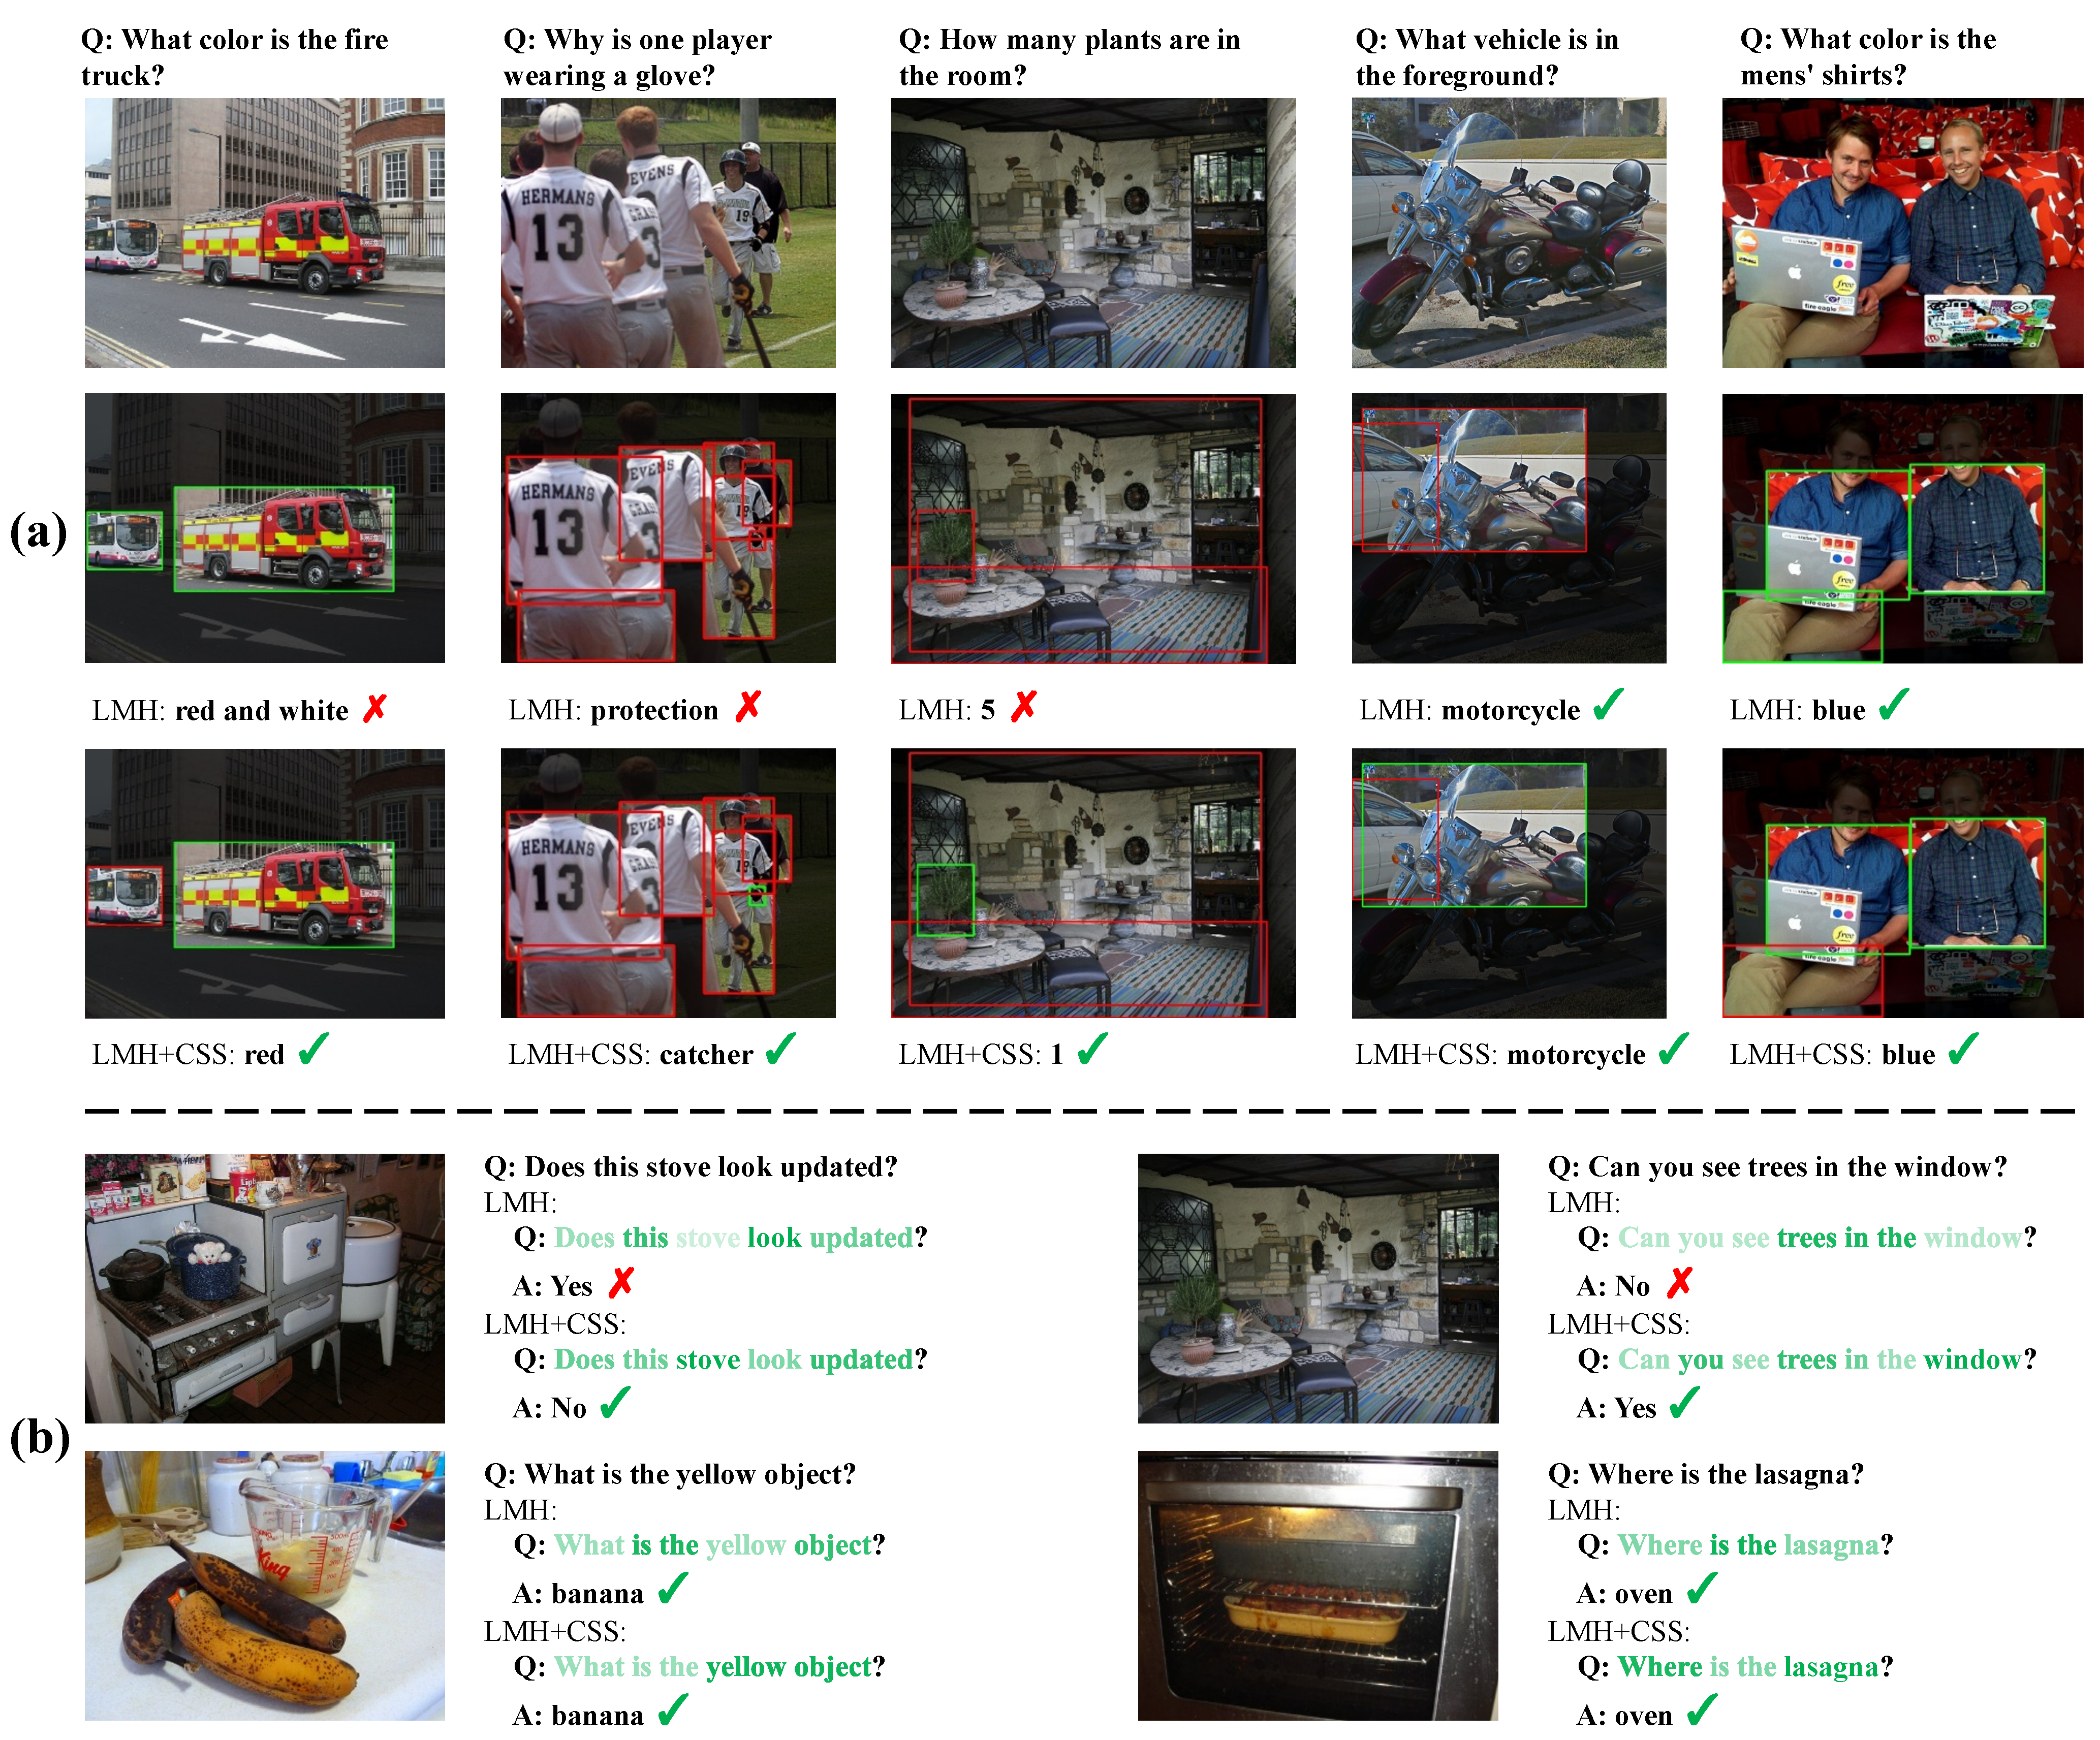
\includegraphics[width=0.95\linewidth]{chapter4/res/visualization.pdf}
    \caption{模型CMAT和模型MOTIFS在数据集Visual Genome上的场景图生成结果对比}
    \label{ch4:fig:visualization}
\end{figure}

\textbf{\kaishu{定性性能对比}}:图~\ref{ch4:fig:visualization}展示了模型CMAT和模型MOTIFS在数据集Visual Genome上的场景图生成结果。其中绿色框表示与真实物体框交叉比大于0.5的物体框,蓝色框表示模型的检测框但数据集中没有标注,红色框表示遗漏的真实物体框。绿色的边表示真阳性(true positive)的视觉关系预测,红色边表示假阴性(false negative)的视觉关系预测,以及蓝色边表示假阳性(false positive)的视觉关系预测。

由图~\ref{ch4:fig:visualization}前两排结果看出可以看出,模型CMAT很少遗漏一些重要的物体节点,如“laptop”、“surfboard”等。这主要原因是模型CMAT的优化目标满足整体一致性,往往对重要的物体节点赋予的权重更大。从第三排结果可以看出,模型CMAT的错误主要是检测出比模型MOTIFS更多的未标注的视觉关系(即蓝色边)。由于目前使用的评价指标主要是基于Recall@K,它只依据所有标注的视觉三元组的排序结果。因此,如果检测出更多的未标注的正样本,反而会得到更低的评价分数。


\section{本章小结}

在本章,我们提出图像场景图生成模型的优化目标应该同时具备整体一致性和局部敏感性。然而,现有的场景图生成模型基本都是使用所有物体和视觉关系分类的交叉熵之和作为模型的优化目标,缺乏整体一致性。为了解决这一问题,本章提出全新的反事实多智能体学习模型(CMAT)。模型CMAT首次将图像场景图生成任务转化成一个多智能体协同合作的决策问题,然后使用场景图生成的评价指标(如Recall@K)作为模型的优化目标,满足整体一致性要求。其次,模型CMAT中包含一个反事实基准模型,通过固定其他智能体的预测同时改变目标智能体的预测,来近似计算每个智能体的局部贡献,进而为每个智能体计算得到更加有效的训练信号。在大规模图像场景图生成数据集Visual Genome上的多个实验设定中,模型CMAT都可以通过提升物体类别的准确率,显著提升场景图生成质量。
